\subsection[Temps]{Approche temporelle.}
\begin{frame}
    \frametitle{Situation initiale.}
    \only<1> {
        \begin{center}
            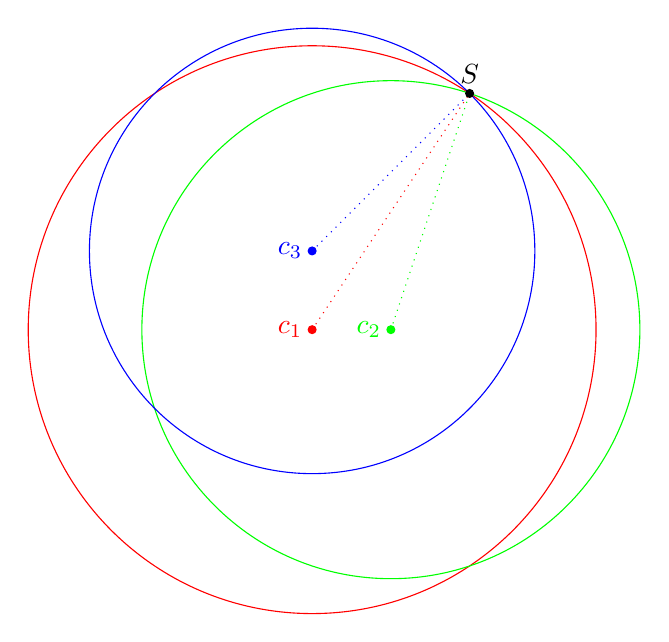
\begin{tikzpicture}
                \filldraw[red] (0,0) circle [radius=.05] node [left] {$c_1$};
                \filldraw[green] (1,0) circle [radius=.05] node [left] {$c_2$};
                \filldraw[blue] (0,1) circle [radius=.05] node [left] {$c_3$};
                \draw[red] (0,0) circle [radius=3.6056];
                \draw[green] (1,0) circle [radius=3.1623];
                \draw[blue] (0,1) circle [radius=2.8284];
                \draw[red,dotted] (0,0) -- (2,3);
                \draw[green,dotted] (1,0) -- (2,3);
                \draw[blue,dotted] (0,1) -- (2,3);
                \filldraw[black] (2,3) circle [radius=.05] node [above] {$S$};
            \end{tikzpicture}
        \end{center}
    }
    \only<2->{ \begin{block}{Équation de départ.}
            \begin{center}
                \begin{tabular}{rcl}
                    $(x-x_1)^2+(y-y_1)^2+(z-z_1)^2$ & $=$ & $d_1^2$ \\
                    $(x-x_2)^2+(y-y_2)^2+(z-z_2)^2$ & $=$ & $d_2^2$ \\
                    $(x-x_3)^2+(y-y_3)^2+(z-z_3)^2$ & $=$ & $d_3^2$ \\
                \end{tabular}
            \end{center}
    \end{block} }
    \only<3-> { \begin{block}{Positionnement des capteurs.}
            \begin{center}
                \begin{tabular}{rcl}
                    $(x_1;y_1;z_1)$ & $=$ & $(0;0;0)$ \\
                    $(x_2;y_2;z_2)$ & $=$ & $(d;0;0)$ \\
                    $(x_3;y_3;z_3)$ & $=$ & $(0;d;0)$ \\
                \end{tabular}
            \end{center}
    \end{block} }
\end{frame}

\begin{frame}
    \frametitle{Résultats.}
    \begin{block}{Triangulation.}
        \begin{center}
            \begin{tabular}{rcl}
                $x$ & $=$ & $\frac{d_1^2-d_2^2+d^2}{2d}$ \\
                $y$ & $=$ & $-\frac{d_3^2-d_1^2-d^2}{2d}$ \\
                $z$ & $=$ & $\pm\sqrt{d_1^2-x^2-y^2}$ \\
            \end{tabular}
        \end{center}
    \end{block}
    \only<2-> {
        \begin{exampleblock}{Simulation.}
            \begin{itemize}
                \pause \item Ordre de grandeur des durées : $10^{-8}s$.
                \pause \item Précision temporelle nécessaire pour un positionnement à $50cm$ : $10^{-11}s$.
            \end{itemize}
        \end{exampleblock}
    }
\end{frame}

\subsection[Intensité]{Utilisation de l'intensité.}
\begin{frame}
    \frametitle{Principe.}
    \begin{exampleblock}{Loi du carré inverse.}
        L'intensité d'un signal électromagnétique est inversement proportionnel au carré de la distance parcourue.
    \end{exampleblock}
    \only<2-> { \begin{block}{Lien entre distance et intensité.}
            \[ \frac{I_1}{I_2} = \frac{d_2^2}{d_1^2} \Leftrightarrow \frac{d_2}{d_1} = \sqrt{\frac{I_1}{I_2}} \]
    \end{block} }
\end{frame}

\subsection[Caméra]{Utilisation d'une caméra.}
\begin{frame}
    \frametitle{Suivi de couleur.}
    \begin{tabular}{cc}
        \includegraphics[width=.4\linewidth]{rcs/follow_bef.png} & \includegraphics[width=.4\linewidth]{rcs/follow_aft.png} \\
    \end{tabular}
    \only<2-> { \begin{alertblock}{Limites}
            \begin{itemize}
                \pause \item L'utilisateur doit être dans le champ de vision du robot.
                \pause \item Il doit porter une couleur particulière.
                \pause \item Relativement sensible à l'éclairage.
                \pause \item Si la couleur est présente ailleurs sur le décor, le robot va être désorienté.
            \end{itemize}
    \end{alertblock} }
\end{frame}

\begin{frame}
    \frametitle{Espace de couleur \emph{HSV}.}
    \begin{center}
        \includegraphics[width=.8\linewidth]{rcs/hsv.png}
    \end{center}
\end{frame}

